\lstdefinestyle{routines-sql}{
    language=SQL,
    basicstyle=\ttfamily\footnotesize,
    breakatwhitespace=true,
    showstringspaces=false,
    upquote=true,
    literate=
        {А}{{\CYRA}}1 {Б}{{\CYRB}}1 {В}{{\CYRV}}1 {Г}{{\CYRG}}1 {Д}{{\CYRD}}1 {Е}{{\CYRE}}1 {Ж}{{\CYRZH}}1 {З}{{\CYRZ}}1 {И}{{\CYRI}}1
        {Й}{{\CYRISHRT}}1 {К}{{\CYRK}}1 {Л}{{\CYRL}}1 {М}{{\CYRM}}1 {Н}{{\CYRN}}1 {О}{{\CYRO}}1 {П}{{\CYRP}}1 {Р}{{\CYRR}}1 {С}{{\CYRS}}1 {Т}{{\CYRT}}1
        {У}{{\CYRU}}1 {Ф}{{\CYRF}}1 {Х}{{\CYRH}}1 {Ц}{{\CYRC}}1 {Ч}{{\CYRCH}}1 {Ш}{{\CYRSH}}1 {Щ}{{\CYRSHCH}}1 {Ъ}{{\CYRHRDSN}}1 {Ы}{{\CYRERY}}1 {Ь}{{\CYRSFTSN}}1
        {Э}{{\CYREREV}}1 {Ю}{{\CYRYU}}1 {Я}{{\CYRYA}}1 {а}{{\cyra}}1 {б}{{\cyrb}}1 {в}{{\cyrv}}1 {г}{{\cyrg}}1 {д}{{\cyrd}}1 {е}{{\cyre}}1
        {ж}{{\cyrzh}}1 {з}{{\cyrz}}1 {и}{{\cyri}}1 {й}{{\cyrishrt}}1 {к}{{\cyrk}}1 {л}{{\cyrl}}1 {м}{{\cyrm}}1 {н}{{\cyrn}}1 {о}{{\cyro}}1 {п}{{\cyrp}}1
        {р}{{\cyrr}}1 {с}{{\cyrs}}1 {т}{{\cyrt}}1 {у}{{\cyru}}1 {ф}{{\cyrf}}1 {х}{{\cyrh}}1 {ц}{{\cyrc}}1 {ч}{{\cyrch}}1 {ш}{{\cyrsh}}1 {щ}{{\cyrshch}}1
        {ъ}{{\cyrhrdsn}}1 {ы}{{\cyrery}}1 {ь}{{\cyrsftsn}}1 {э}{{\cyrerev}}1 {ю}{{\cyryu}}1 {я}{{\cyrya}}1
}

\newpage
\noindent
{\Large \textbf{\section[Лабораторная работа №5 <<Функции и процедуры>>]{Лабораторная работа №5\\<<Функции и процедуры>>}}} \par

\subsection{Задачи}

\begin{enumerate}
    \item Реализовать функцию формирования фамилии с инициалами сотрудника, при этом необходимо обрабатывать возможное отсутствие отчества. 
    \item Реализовать процедуру назначения сотрудника куратором выставки. Аргументами процедуры являются исходные атрибуты представления и обязательные атрибуты связанных таблиц.
    Если значение какого-либо атрибута не было найдено в исходных таблицах, то необходимо выполнить вставку нового значения.
\end{enumerate}

\subsection{Создание функции} \noindent

Функция \texttt{employee\_initials} принимает фамилию, имя и отчество и возвращает фамилию с инициалами. 
При отсутствии отчества в результате формируется только фамилия и инициал имени. Исходный текст приведен в Приложении~А (Листинг~\ref{lst:employee-initials}). \par

Для демонстрации выполнен запрос к таблице \texttt{employees} (см.Листинг~\ref{lst:employee-initials-query}). Результат приведен на Рис.~\ref{fig:employee-initials-result}. \par

\hspace{7pt}
\begin{lstlisting}[style=routines-sql, caption={Запрос с применением функции employee\_initials}, label={lst:employee-initials-query}]
SELECT last_name AS "Имя", first_name AS "Фамилия", middle_name AS "Отчество",
       employee_initials(last_name, first_name, middle_name) AS "ФИО"
FROM employees;
\end{lstlisting}

\begin{figure}[H]
    \centering
    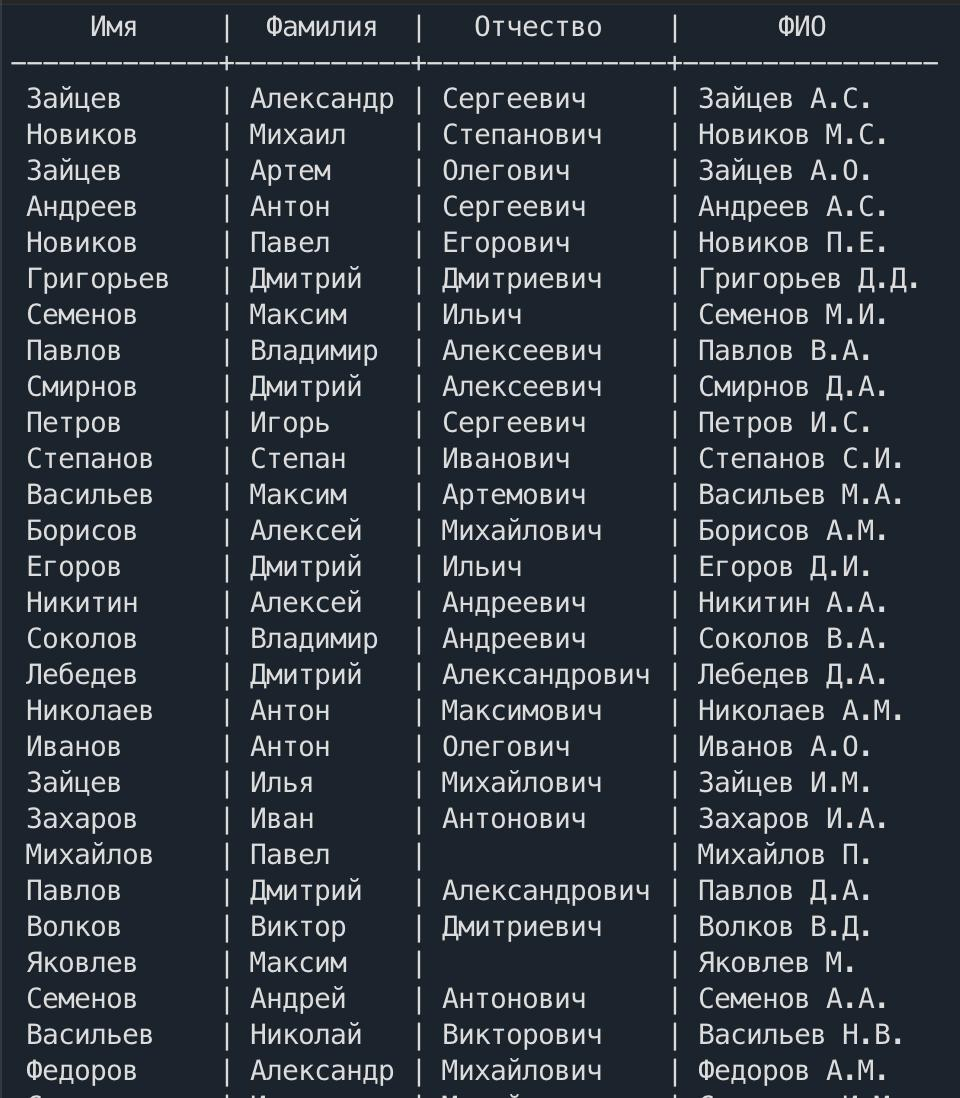
\includegraphics[width=1\textwidth,height=0.6\textheight,keepaspectratio]{pic/function_result.jpg}
    \caption{Результата запроса с применением функции employee\_initials}
    \label{fig:employee-initials-result}
\end{figure}



\subsection{Создание процедуры} \noindent

Процедура \texttt{assign\_exhibition\_curator} принимает фамилию, имя и отчество сотрудника, название выставки и название ее типа.
Число курируемых выставок и число их типов являются расчетными атрибутами, поэтому они не являются аргументами процедуры. \par

Сотрудник определяется по фамилии, имени и отчеству, тип выставки - по названию, выставка - по названию и найденному типу. Если записей о сотруднике, типе выставки или выставке нет, то соответствующие записи добавляются в таблицы \texttt{employees}, \texttt{exhibition\_type} и \texttt{exhibitions}. Если рассматриваемый сотрудник еще не курирует данную выставку, то в таблицу \CuratorsTable{} добавляется запись о назначении кураторства. Повторный вызов для той же пары сотрудника и выставки не создает повторную запись о кураторстве. \par

\hspace{8pt}

Блок-схема, реализующая логику процедуры, приведена на Рис.~\ref{fig:curator-procedure}. Исходный текст процедуры приведен в Приложении~Б (Листинг~\ref{lst:assign-exhibition-curator}). \par

\begin{figure}[H]
    \centering
    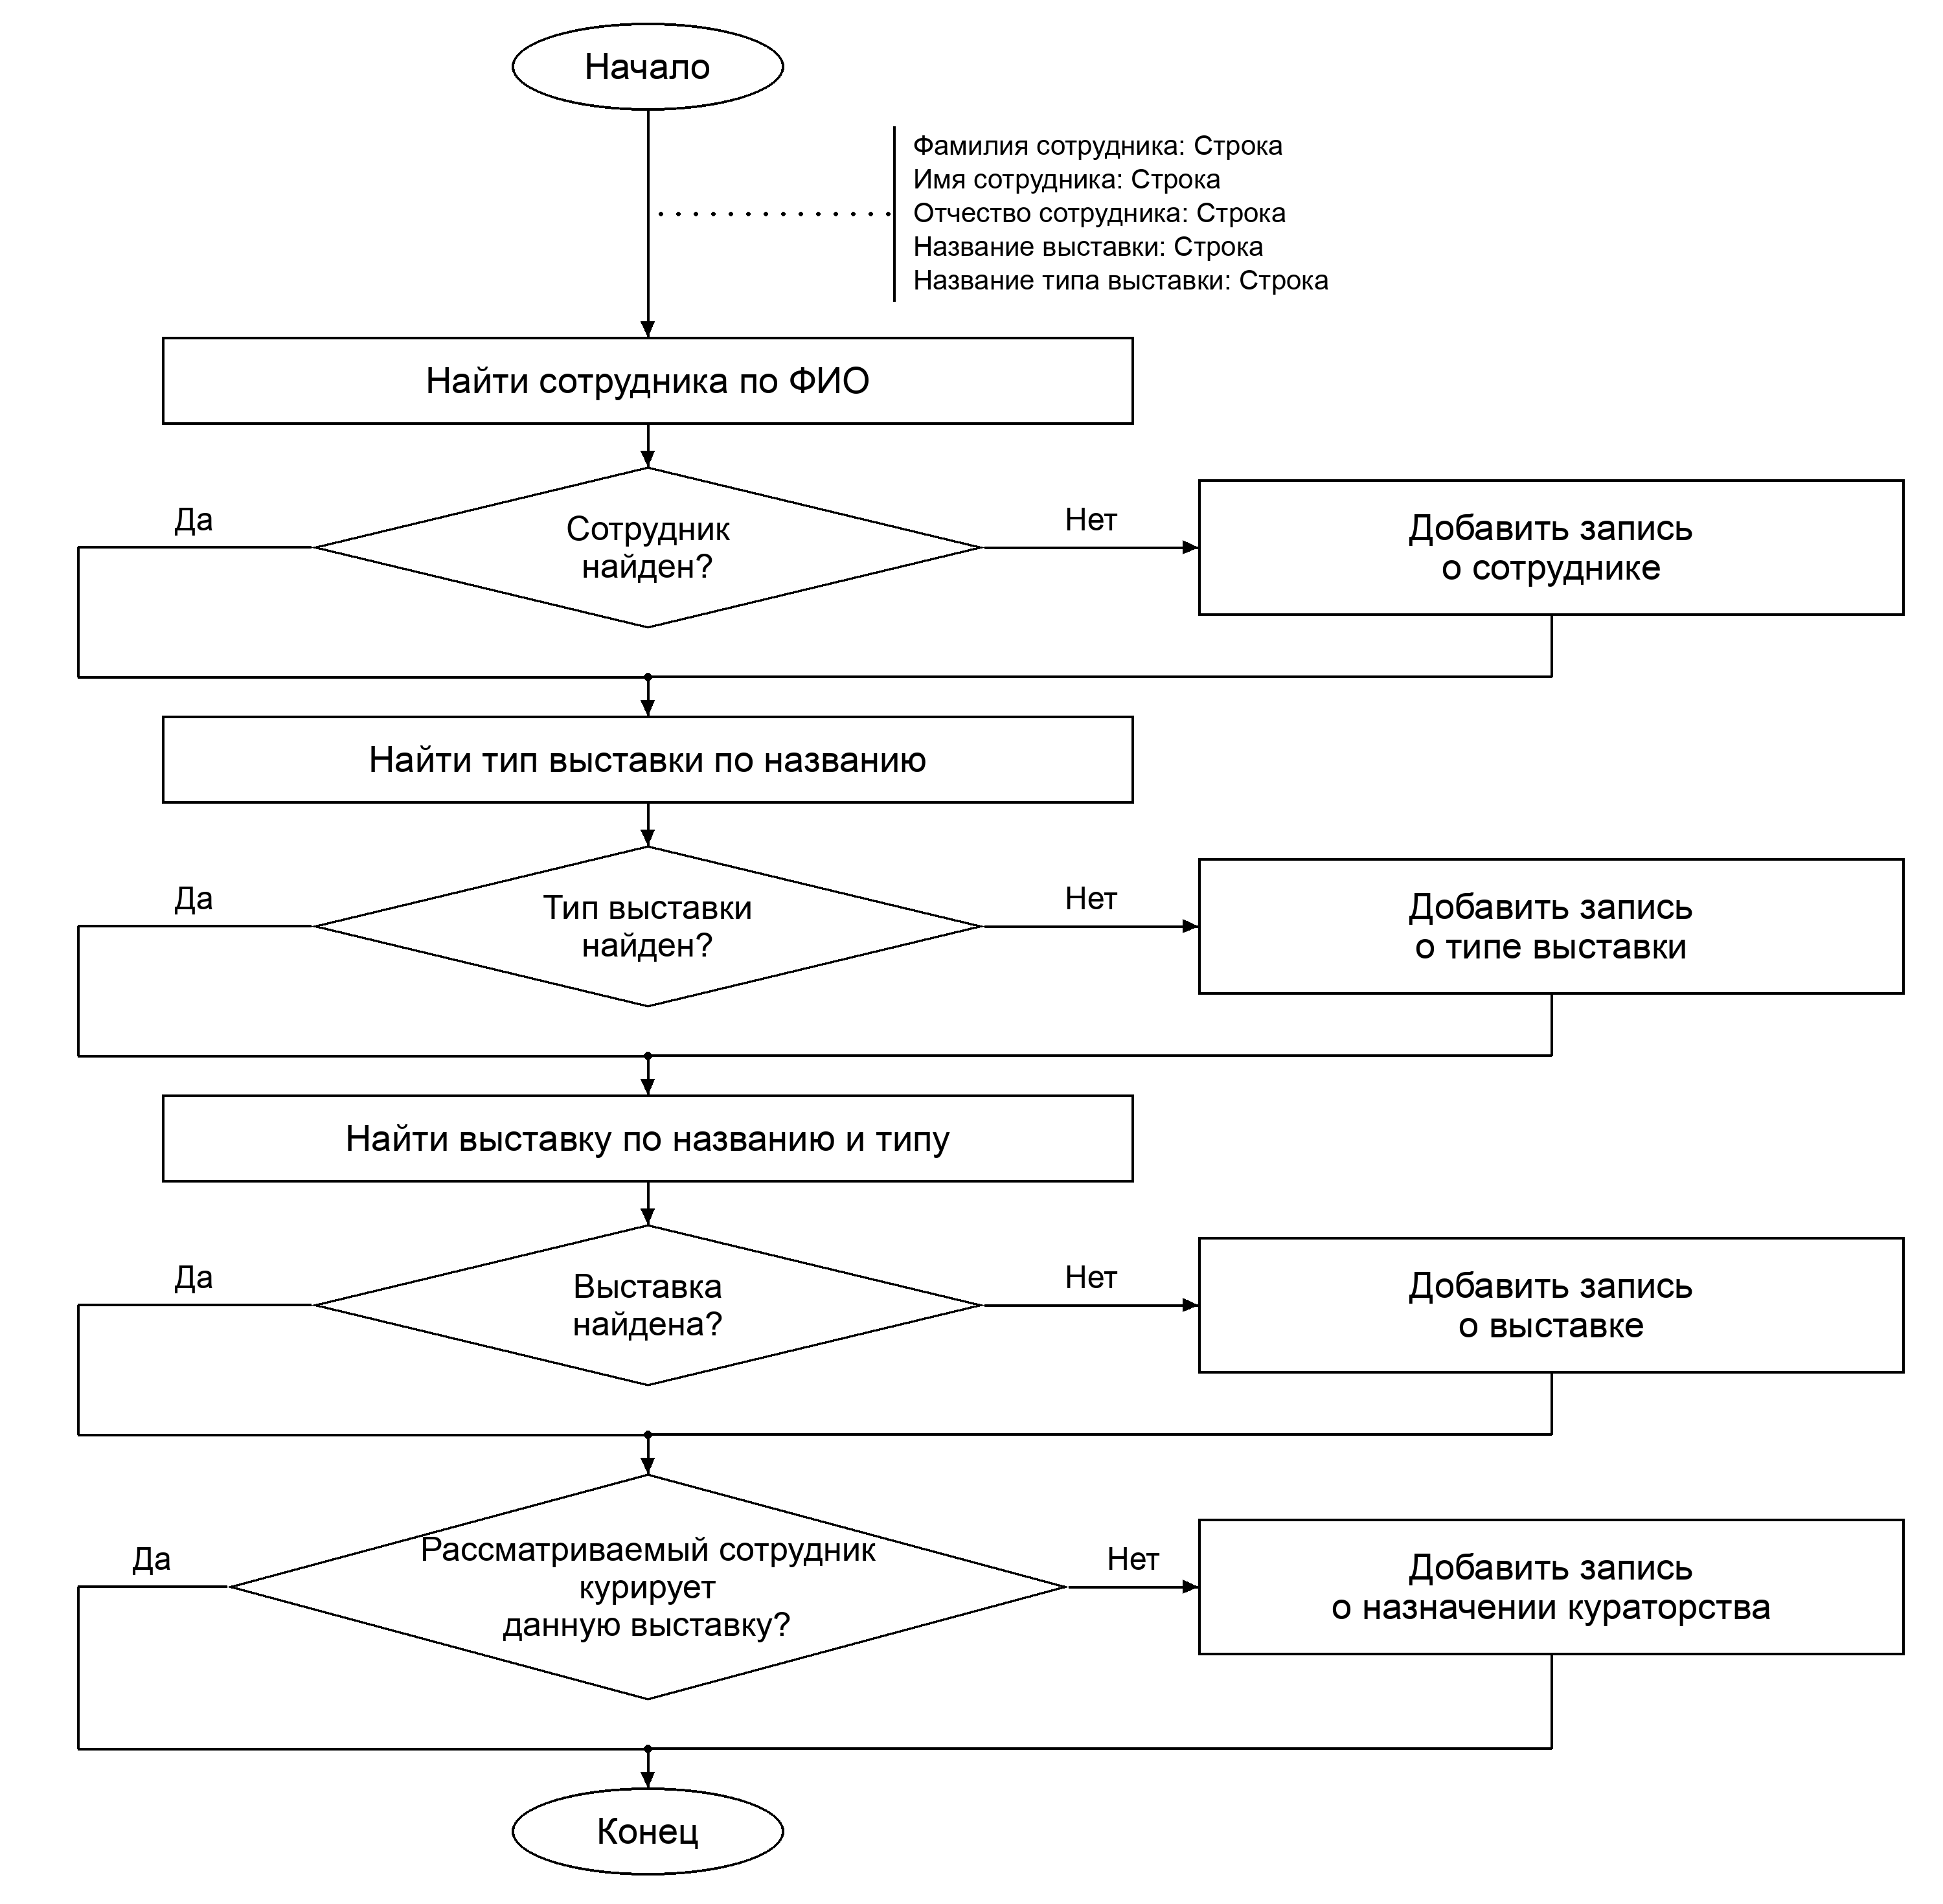
\includegraphics[width=\textwidth,height=0.70\textheight,keepaspectratio]{pic/curator_procedure.png}
    \caption{Блок-схема процедуры назначения сотрудника куратором выставки}
    \label{fig:curator-procedure}
\end{figure}


\subsection{Проверка процедуры}

Для проверки процедуры используются типы выставок <<ЛР5 Тип А>> и <<ЛР5 Тип Б>>. Исходные состояния представлены в Таблице~\ref{tab:curator-procedure-cases}. \par

\begin{table}[H]
\centering
\caption{Примеры для проверки работы процедуры}
\label{tab:curator-procedure-cases}
\begin{tabularx}{\textwidth}{|c|L|}
\hline
\textbf{№} & \textbf{Описание проверяемого состояния} \\
\hline
1 & Сотрудник, выставка и ее тип отсутствуют. \\
\hline
2 & Сотрудник и выставка существуют. Сотрудник уже курирует эту выставку. \\
\hline
3 & Сотрудник отсутствует, выставка существует. \\
\hline
4 & Сотрудник существует, выставка и ее тип отсутствуют. \\
\hline
5 & Сотрудник и выставка существуют. Кураторство отсутствует. После назначения число курируемых выставок увеличивается с четырех до пяти, число типов остается равным одному. \\
\hline
6 & Сотрудник и выставка существуют. Кураторство отсутствует. После назначения на выставку другого типа число выставок увеличивается с четырех до пяти, число типов - с одного до двух. \\
\hline
\end{tabularx}
\end{table}

Исходные состояния и результаты применения процедуры приведены в Таблице~\ref{tab:curator-procedure-comparison}. \par

\storeareas\RoutinesSavedValues
\clearpage
\KOMAoptions{
    paper=a2,
    paper=landscape,
    DIV=36,
    BCOR=0mm,
    pagesize
}
\recalctypearea

\begingroup
\large
\setlength{\tabcolsep}{8pt}
\setlength{\extrarowheight}{5pt}
\setlength{\shotunit}{0.32pt}
\setlength{\shotmax}{0.462\textwidth}
\begin{longtable}{|>{\centering\arraybackslash}p{1cm}|>{\centering\arraybackslash}p{0.462\textwidth}|>{\raggedright\arraybackslash}p{0.462\textwidth}|}
\caption{Исходные состояния и результаты применения процедуры}
\label{tab:curator-procedure-comparison} \\
\hline
\textbf{№} & \textbf{Исходное состояние} & {\centering\textbf{Результат применения процедуры}\par} \\
\hline
\endfirsthead
\hline
\textbf{№} & \textbf{Исходное состояние} & {\centering\textbf{Результат применения процедуры}\par} \\
\hline
\endhead
% Слева: \includegraphics[width=\linewidth,height=50mm,keepaspectratio]{pic/имя_файла.png}
% Справа после текста: \par\smallskip{\centering\includegraphics[width=\linewidth,height=42mm,keepaspectratio]{pic/имя_файла.png}\par}
1 &
Сотрудник Тест Тестов Тестович, выставка <<ЛР5 Выставка А>> и тип <<ЛР5 Тип А>> отсутствуют. \par\smallskip
\shot{proc1_1.jpg}{1596}{0}{0}\par\smallskip
\shot{proc1_2.jpg}{1110}{0}{0}\par\smallskip
\shot{proc1_3.jpg}{2006}{0}{0}
&
В таблицы \texttt{employees}, \texttt{exhibition\_type} и \texttt{exhibitions} добавлены записи о сотруднике, типе выставки и выставке. В \CuratorsTable{} добавлена запись о назначении сотрудника куратором выставки. В таблице статистики по кураторам появилась строка сотрудника. Сотрудник курирует одну выставку одного типа, поэтому оба счетчика равны одному. \par\smallskip
{\centering
\shot{proc1_4.png}{1682}{0}{0}\par\smallskip
\shot{proc1_5.jpg}{1614}{0}{0}\par\smallskip
\shot{proc1_6.jpg}{1090}{0}{0}\par\smallskip
\shot{proc1_7.jpg}{2002}{0}{0}\par}
\\
\hline
2 &
Тест Тестов Тестович уже курирует выставку <<ЛР5 Выставка А>>. Сотрудник курирует одну выставку одного типа. \par\smallskip
\shot{proc2_1.jpg}{1606}{0}{0}\par\smallskip
\shot{proc2_2.jpg}{1102}{0}{0}\par\smallskip
\shot{proc2_3.jpg}{2002}{0}{0}
&
Повторный вызов использует существующие записи о сотруднике, типе выставки и выставке. Поскольку сотрудник уже курирует эту выставку, новая запись о кураторстве не добавляется. Идентификаторы сотрудника и выставки, а также число записей в результатах запросов не изменились. Сотрудник по-прежнему курирует одну выставку одного типа, поэтому оба счетчика остаются равными одному. \par\smallskip
{\centering
\shot{proc2_4.png}{1704}{0}{0}\par\smallskip
\shot{proc2_5.jpg}{1602}{0}{0}\par\smallskip
\shot{proc2_6.jpg}{1116}{0}{0}\par\smallskip
\shot{proc2_7.jpg}{1998}{0}{0}\par}
\\
\hline
3 &
Выставка <<ЛР5 Выставка А>> существует. Сотрудник Тестов Павел Павлович отсутствует. \par\smallskip
\shot{proc3_1.jpg}{1610}{0}{0}\par\smallskip
\shot{proc3_2.jpg}{1096}{0}{0}\par\smallskip
\shot{proc3_3.jpg}{1998}{0}{0}
&
В таблицу \texttt{employees} добавлен сотрудник Тестов Павел Павлович. Для типа выставки и выставки использованы существующие записи. В \CuratorsTable{} зарегистрировано кураторство нового сотрудника над выставкой. В таблице статистики по кураторам появилась его строка: число курируемых выставок и число их типов равны одному. Идентификатор выставки и сведения о ней не изменились. \par\smallskip
{\centering
\shot{proc3_4.png}{1722}{0}{0}\par\smallskip
\shot{proc3_5.jpg}{1622}{0}{0}\par\smallskip
\shot{proc3_6.jpg}{1088}{0}{0}\par\smallskip
\shot{proc3_7.jpg}{2002}{0}{0}\par}
\\
\hline
4 &
Тест Тестов Тестович курирует выставку <<ЛР5 Выставка А>>. Выставка <<ЛР5 Выставка Б>> и тип <<ЛР5 Тип Б>> отсутствуют. \par\smallskip
\shot{proc4_1.jpg}{1612}{0}{0}\par\smallskip
\shot{proc4_2.jpg}{1114}{0}{0}\par\smallskip
\shot{proc4_3.jpg}{2002}{0}{0}
&
Для сотрудника использована существующая запись. В таблицы \texttt{exhibition\_type} и \texttt{exhibitions} добавлены новый тип и выставка. В \CuratorsTable{} зарегистрировано кураторство сотрудника над новой выставкой. Число курируемых выставок увеличилось с 1 до 2, число их типов также увеличилось с 1 до 2. Запись о сотруднике не изменилась. \par\smallskip
{\centering
\shot{proc4_4.png}{1718}{0}{0}\par\smallskip
\shot{proc4_5.jpg}{1588}{0}{0}\par\smallskip
\shot{proc4_6.jpg}{1092}{0}{0}\par\smallskip
\shot{proc4_7.jpg}{1998}{0}{0}\par}
\\
\hline
5 &
Тестов Алексей Алексеевич курирует четыре выставки одного типа. Выставка <<ЛР5 Выставка А>> того же типа существует, но сотрудник ее еще не курирует. \par\smallskip
\shot{proc5_1.jpg}{1606}{0}{0}\par\smallskip
\shot{proc5_2.jpg}{1096}{0}{0}\par\smallskip
\shot{proc5_3.jpg}{1994}{0}{0}
&
Для сотрудника, типа выставки и выставки использованы существующие записи. Добавлена запись о назначении сотрудника куратором выставки <<ЛР5 Выставка А>>. Число курируемых выставок увеличилось с 4 до 5. Число их типов осталось равным 1, поскольку пятая выставка относится к тому же типу, что и остальные. Записи о сотруднике и выставке не изменились. \par\smallskip
{\centering
\shot{proc5_4.png}{1774}{0}{0}\par\smallskip
\shot{proc5_5.jpg}{1606}{0}{0}\par\smallskip
\shot{proc5_6.jpg}{1096}{0}{0}\par\smallskip
\shot{proc5_7.jpg}{2008}{0}{0}\par}
\\
\hline
6 &
Тестов Алексей Алексеевич курирует четыре выставки одного типа. Выставка <<ЛР5 Выставка Б>> другого типа существует, но сотрудник ее еще не курирует. \par\smallskip
\shot{proc6_1.jpg}{1616}{0}{0}\par\smallskip
\shot{proc6_2.jpg}{1100}{0}{0}\par\smallskip
\shot{proc6_3.jpg}{1998}{0}{0}
&
Для сотрудника, типа выставки и выставки использованы существующие записи. Добавлена запись о назначении сотрудника куратором выставки <<ЛР5 Выставка Б>>. Число курируемых выставок увеличилось с 4 до 5. Число их типов увеличилось с 1 до 2, поскольку сотрудник впервые назначен куратором выставки этого типа. Записи о сотруднике и выставке не изменились. \par\smallskip
{\centering
\shot{proc6_4.png}{1788}{0}{0}\par\smallskip
\shot{proc6_5.jpg}{1614}{0}{0}\par\smallskip
\shot{proc6_6.jpg}{1094}{0}{0}\par\smallskip
\shot{proc6_7.jpg}{1996}{0}{0}\par}
\\
\hline
\end{longtable}
\endgroup

\clearpage
\RoutinesSavedValues
\recalctypearea
